\documentclass[11pt]{article}
\usepackage[margin=1in]{geometry}
\usepackage{amsmath}
\usepackage{booktabs}
\usepackage{tikz}
\usepackage{hyperref}

\title{A Field Guide to \LaTeX{} Sorcery}
\author{A. Apprentice \\ \small Department of Arcane Typesetting}
\date{Walpurgis Night}

\begin{document}
\maketitle

\begin{abstract}
Every \LaTeX{} user eventually casts a spell they do not understand. This
guide catalogues the common incantations, the curses they summon, and the
counter-charms that banish them.
\end{abstract}

\section{Incantations}
\label{sec:incantations}

The oldest spells are still the strongest~\cite{knuth}. A well-formed
incantation balances its braces and names its environment:
\begin{equation}
  \mathcal{P}(\text{compiles}) = \prod_{i=1}^{n} \left(1 - \varepsilon_i\right),
  \label{eq:success}
\end{equation}
where $\varepsilon_i$ is the chance that the $i$-th package disagrees with
the rest. Equation~\eqref{eq:success} explains why every new package is a
small act of faith.

\begin{figure}[h]
  \centering
  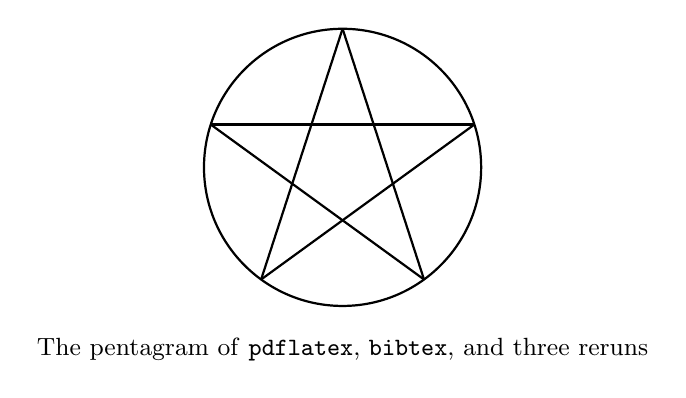
\begin{tikzpicture}[scale=1.1]
    \draw[thick] (0,0) circle (1.6);
    \foreach \a in {90,162,234,306,18}
      \draw[thick] (\a:1.6) -- ({\a+144}:1.6);
    \node at (0,-2.1) {\small The pentagram of \texttt{pdflatex}, \texttt{bibtex}, and three reruns};
  \end{tikzpicture}
  \caption{A standard summoning circle.}
  \label{fig:circle}
\end{figure}

\section{Curses and counter-charms}
\label{sec:curses}

Table~\ref{tab:curses} lists the curses most often reported by
apprentices~\cite{lamport}, with the counter-charm that lifts each one.

\begin{table}[h]
  \centering
  \begin{tabular}{@{}lll@{}}
    \toprule
    Curse & Symptom & Counter-charm \\
    \midrule
    Undefined control sequence & A typo in a command & Check the spelling \\
    Missing \verb|$| inserted & Math outside math mode & Wrap it in \verb|$...$| \\
    Runaway argument & A brace left open & Count your braces \\
    Overfull \verb|\hbox| & A line that will not break & Rephrase, or \verb|\sloppy| \\
    \bottomrule
  \end{tabular}
  \caption{Common curses, as seen in Section~\ref{sec:incantations}.}
  \label{tab:curses}
\end{table}

Figure~\ref{fig:circle} remains the safest way to call the engine.


\begin{thebibliography}{9}
\bibitem{knuth} D.~E. Knuth. \emph{The \TeX book}. Addison-Wesley, 1984.
\bibitem{lamport} L.~Lamport. \emph{\LaTeX: A Document Preparation System}. Addison-Wesley, 1994.
\end{thebibliography}

\end{document}
